\section{Визуализация и анализ данных в Yandex DataLens}

Настоящий раздел описывает процесс подключения базы данных ClickHouse к облачной BI-платформе Yandex DataLens, формирование датасета с вычисляемыми полями, расчёт ключевых метрик эффективности рекламных кампаний и проведение базового анализа по рекламодателям.

\subsection{Подключение ClickHouse к DataLens}
\label{subsec:datalens_connection}

Yandex DataLens является облачным сервисом и требует сетевой доступности источника данных из публичного интернета. Поскольку сервер ClickHouse развёрнут локально, прямое подключение из DataLens к нему невозможно без дополнительных средств проброса сети.

Для решения данной задачи применялся инструмент \texttt{ngrok}~\cite{ngrok}, осуществляющий проброс локального порта через защищённый HTTPS-туннель. 

Подключение DataLens к базе данных настроено с использованием TLS-сертификата и парольной аутентификации, что обеспечивает минимальные требования безопасности при работе с публично доступным туннелем. Интерфейс настройки подключения представлен на Рисунке~\ref{fig:datalens_connection}.

\begin{figure}[h!]
    \centering
    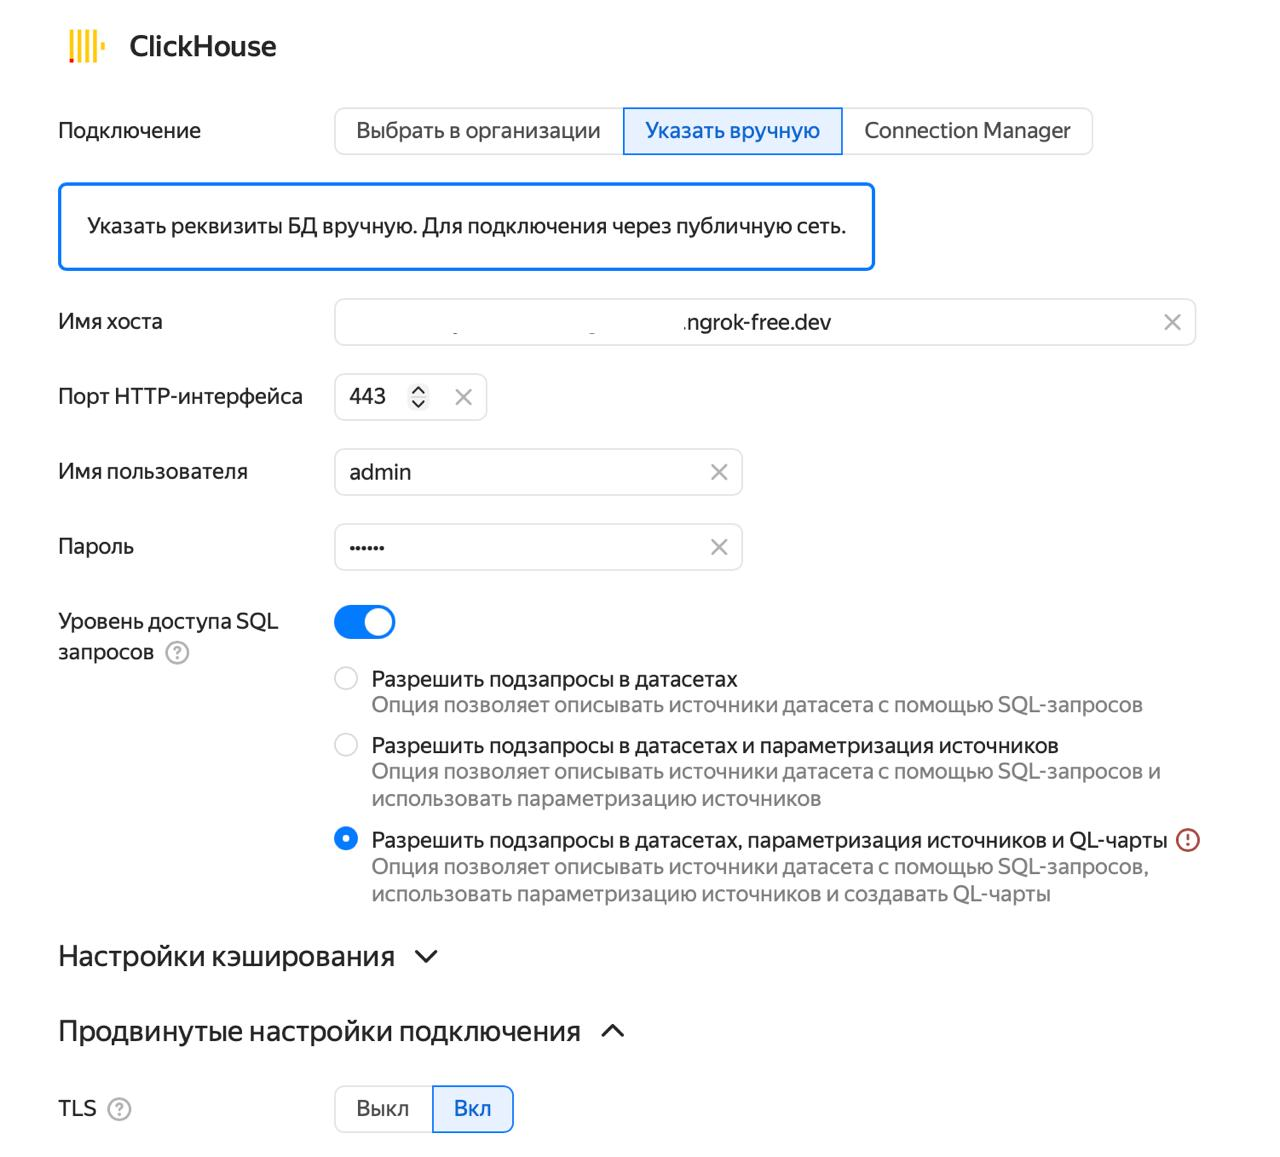
\includegraphics[width=0.82\textwidth]{images/connection.jpeg}
    \caption{Настройка подключения ClickHouse в интерфейсе Yandex DataLens.}
    \label{fig:datalens_connection}
\end{figure}

\subsection{Формирование датасета}
\label{subsec:datalens_dataset}

\subsubsection*{Понятие датасета в DataLens}

Датасет в Yandex DataLens представляет собой логическое описание источника данных: он определяет набор таблиц, связи между ними и перечень полей, доступных для построения чартов. Датасет является промежуточным слоем между физическим хранилищем (ClickHouse) и визуализациями: все вычисляемые поля, созданные на уровне датасета, автоматически становятся доступными во всех чартах, построенных на его основе.

\subsubsection*{Источники данных и схема связей}

Основным источником данных в датасете является таблица \texttt{ads\_data}, сформированная на этапе подготовки данных (см. подраздел~\ref{subsec:ads_data}). Поля \texttt{region\_id} и \texttt{city\_id} в данной таблице хранят числовые идентификаторы, не несущие смысловой нагрузки при визуализации. Для их декодирования в читаемые названия в ClickHouse были созданы две справочные таблицы: \texttt{ipinyou\_db.cities} и \texttt{ipinyou\_db.regions}. DDL-определения обеих таблиц приведены в Приложении~\ref{app:ddl_dicts}.

Связи между таблицами настраивались непосредственно в интерфейсе датасета DataLens без написания SQL-запросов. К таблице \texttt{ads\_data} были добавлены два LEFT JOIN:

\begin{itemize}
    \item \texttt{ads\_data.city\_id = ipinyou\_db.cities.city\_id} --- для получения поля \texttt{city\_name};
    \item \texttt{ads\_data.region\_id = ipinyou\_db.regions.region\_id} --- для получения поля \texttt{region\_name}.
\end{itemize}

Использование LEFT JOIN гарантирует сохранение всех строк основной таблицы: записи с отсутствующим или неизвестным идентификатором города или региона не исключаются из анализа, а соответствующие поля принимают значение \texttt{NULL}. Схема связей датасета представлена на Рисунке~\ref{fig:datalens_dataset}.

\begin{figure}[h!]
    \centering
    
\includegraphics[width=0.72\textwidth]{images/dataset.jpeg}
    \caption{Схема связей датасета в интерфейсе Yandex DataLens: \texttt{ads\_data} ← LEFT JOIN → \texttt{regions}, \texttt{cities}.}
    \label{fig:datalens_dataset}
\end{figure}

\subsubsection*{Вычисляемые поля уровня датасета}

DataLens позволяет создавать вычисляемые поля как на уровне датасета, так и на уровне отдельного чарта. Принципиальное различие состоит в следующем: поле, созданное в датасете, доступно во всех чартах, построенных на его основе, тогда как поле уровня чарта существует только в рамках одного конкретного виджета. Поскольку базовые агрегаты и метрики используются в нескольких визуализациях, они были вынесены на уровень датасета.

Первым шагом были определены агрегирующие поля, соответствующие основным событиям RTB-воронки:

\begin{itemize}
    \item \texttt{bids} $=$ \texttt{COUNT([bid\_id])} --- общее число ставок DSP;
    \item \texttt{imps} $=$ \texttt{COUNT\_IF([is\_win] = 1)} --- число выигранных аукционов (показов);
    \item \texttt{clicks} $=$ \texttt{COUNT\_IF([is\_clicked] = 1)} --- число кликов по объявлению;
    \item \texttt{convs} $=$ \texttt{COUNT\_IF([is\_conversion] = 1)} --- число конверсий;
    \item \texttt{cost} $=$ \texttt{SUM([paying\_price])} --- суммарные затраты рекламодателя;
    \item \texttt{win\_ratio} $=$ \texttt{[imps] / [bids]} --- доля выигранных аукционов.
\end{itemize}

Дополнительно было создано вычисляемое измерение \texttt{advertiser\_name} с использованием формулы \texttt{CASE}:

\begin{verbatim}
CASE [advertiser_id]
    WHEN 1458 THEN "Advertiser 1458"
    WHEN 3358 THEN "Advertiser 3358"
    WHEN 3386 THEN "Advertiser 3386"
    WHEN 3427 THEN "Advertiser 3427"
    WHEN 3476 THEN "Advertiser 3476"
    ELSE "Unknown"
END
\end{verbatim}

Использование \texttt{CASE} обосновано малым числом уникальных значений \texttt{advertiser\_id} в датасете iPinYou, что делает создание отдельной справочной таблицы избыточным. Формула встраивается непосредственно в датасет и обеспечивает читаемые метки рекламодателей во всех чартах.

\subsection{Расчёт метрик эффективности рекламных кампаний}
\label{subsec:datalens_metrics}

\subsubsection*{Вычисляемые поля метрик}

На уровне датасета были созданы следующие поля метрик эффективности (определения метрик приведены в разделе «Основные термины и определения»):

\begin{itemize}
    \item \texttt{CPM} $=$ \texttt{[cost] / [imps]} --- средняя цена за тысячу показов, юань/CPM;
    \item \texttt{CTR} $=$ \texttt{[clicks] / [imps]} --- показатель кликабельности, доля;
    \item \texttt{CVR} $=$ \texttt{[convs] / [clicks]} --- коэффициент конверсии, доля;
    \item \texttt{eCPC} $=$ \texttt{[cost] / [clicks]} --- эффективная стоимость клика, юань/клик;
    \item \texttt{eCPA} $=$ \texttt{[cost] / [convs]} --- эффективная стоимость конверсии, юань/конверсия.
\end{itemize}

\subsection{Базовый анализ по рекламодателям}
\label{subsec:datalens_analysis}

\subsubsection*{Сводная таблица метрик по рекламодателям}

В качестве первичного аналитического инструмента в DataLens был построен чарт типа «Таблица» с измерением \texttt{advertiser\_name} и всеми рассчитанными мерами: \texttt{bids}, \texttt{imps}, \texttt{clicks}, \texttt{convs}, \texttt{cost}, \texttt{win\_ratio}, \texttt{CPM}, \texttt{CTR}, \texttt{CVR}, \texttt{eCPC}, \texttt{eCPA}. Данная таблица позволяет сопоставить рекламодателей по всем ключевым показателям в едином представлении. Результаты приведены в Таблице~\ref{tab:advertiser_metrics}.

\begin{table}[h!]
\small
\begin{center}
\caption{Сводные метрики эффективности рекламных кампаний по рекламодателям.}
\label{tab:advertiser_metrics}
\renewcommand{\arraystretch}{1.15}
\begin{tabular}{l|r|r|r|r|r|r}
  \textbf{Рекламодатель} & \textbf{Bids} & \textbf{Imps} & \textbf{Clicks} & \textbf{Convs} & \textbf{Win ratio} & \textbf{CTR} \\
  \hline
  Chinese vert. e-com. & 14\,701\,496 & 3\,077\,016 & 2\,450 & 1    & 20,93\% & 0,080\% \\
  Footwear             &  5\,292\,053 & 1\,305\,287 &   823 & 437  & 24,67\% & 0,063\% \\
  Intl. e-commerce     & 14\,091\,931 & 2\,835\,897 & 2\,079 & 0   & 20,12\% & 0,073\% \\
  Milk powder          &  2\,987\,731 &   830\,685 &   279 &  89  & 27,80\% & 0,034\% \\
  Mobile app install   &  1\,017\,927 &   311\,373 & 1\,382 &  0  & 30,59\% & 0,444\% \\
  Oil                  & 14\,032\,619 & 2\,581\,615 & 1\,917 &  0  & 18,40\% & 0,074\% \\
  Software             &  3\,751\,016 & 1\,727\,542 & 1\,367 & 377 & 46,06\% & 0,079\% \\
  Telecom              &  2\,159\,708 &   684\,966 &   207 &  0   & 31,72\% & 0,030\% \\
  Tire                 &  6\,712\,268 & 1\,968\,277 & 1\,025 & 26  & 29,32\% & 0,052\% \\
  \hline
  \textbf{Итого}       & \textbf{64\,746\,749} & \textbf{15\,322\,658} & \textbf{11\,529} & \textbf{930} & \textbf{23,67\%} & \textbf{0,075\%} \\
\end{tabular}
\end{center}
\end{table}

\begin{table}[h!]
\small
\begin{center}
\caption{Ценовые метрики рекламных кампаний по рекламодателям (юань).}
\label{tab:advertiser_cost_metrics}
\renewcommand{\arraystretch}{1.15}
\begin{tabular}{l|r|r|r|r|r}
  \textbf{Рекламодатель} & \textbf{Cost} & \textbf{CPM} & \textbf{CVR} & \textbf{eCPC} & \textbf{eCPA} \\
  \hline
  Chinese vert. e-com. & 211\,938\,121 & 68\,877,81 & 0,041\%  & 86\,505,36    & 211\,938\,121,00 \\
  Footwear             & 116\,696\,494 & 89\,402,94 & 53,098\% & 141\,794,04   & 267\,040,03      \\
  Intl. e-commerce     & 217\,718\,557 & 76\,772,38 & 0,000\%  & 104\,722,73   & ---              \\
  Milk powder          &  77\,273\,250 & 93\,023,53 & 31,900\% & 276\,965,05   & 868\,238,76      \\
  Mobile app install   &  19\,625\,531 & 63\,029,01 & 0,000\%  &  14\,200,82   & ---              \\
  Oil                  & 208\,912\,977 & 80\,923,37 & 0,000\%  & 108\,979,12   & ---              \\
  Software             & 159\,313\,651 & 92\,219,84 & 27,579\% & 116\,542,54   & 422\,582,63      \\
  Telecom              &  61\,372\,941 & 89\,599,98 & 0,000\%  & 296\,487,64   & ---              \\
  Tire                 & 155\,933\,746 & 79\,223,48 & 2,537\%  & 152\,130,48   & 5\,997\,451,77   \\
  \hline
  \textbf{Итого}       & \textbf{1\,228\,785\,268} & \textbf{80\,194,00} & \textbf{8,067\%} & \textbf{106\,582,12} & \textbf{1\,321\,274,48} \\
\end{tabular}
\end{center}
\end{table}

\subsubsection*{Аналитические наблюдения}

Из Таблицы~\ref{tab:advertiser_metrics} и Таблицы~\ref{tab:advertiser_cost_metrics} следует, что рекламодатель «Mobile app install» демонстрирует наименьший CPM среди всех участников (63\,029 юань/CPM) при одновременно высоком \texttt{win\_ratio} (30,59\%). Это свидетельствует об эффективной стратегии ставок: кампания успешно конкурирует на аукционах, не переплачивая за показы. Примечательно, что данный рекламодатель также показывает наибольший CTR (0,444\%) --- в 5--6 раз выше среднего по выборке (0,075\%), что указывает на высокое соответствие рекламного объявления целевой аудитории.

Противоположный профиль демонстрирует рекламодатель «Milk powder»: наибольший CPM (93\,024 юань/CPM) при относительно скромном \texttt{win\_ratio} (27,80\%). Высокая цена показа в сочетании с низким CTR (0,034\%) указывает на агрессивную ценовую стратегию, не подкреплённую соответствующим качеством взаимодействия аудитории с объявлением.

